% -----------------------------------------------
% Template for ICMC SMC 2014
% adapted and corrected from the template for SMC 2013,  which was adapted from that of  SMC 2012, which was adapted from that of SMC 2011
% -----------------------------------------------

\documentclass{article}
\usepackage{icmcsmc2014}
\usepackage{times}
\usepackage{ifpdf}
\usepackage[english]{babel}
%\usepackage{cite}

%%%%%%%%%%%%%%%%%%%%%%%% Some useful packages %%%%%%%%%%%%%%%%%%%%%%%%%%%%%%%
%%%%%%%%%%%%%%%%%%%%%%%% See related documentation %%%%%%%%%%%%%%%%%%%%%%%%%%
%\usepackage{amsmath} % popular packages from Am. Math. Soc. Please use the
%\usepackage{amssymb} % related math environments (split, subequation, cases,
%\usepackage{amsfonts}% multline, etc.)
%\usepackage{bm}      % Bold Math package, defines the command \bf{}
%\usepackage{paralist}% extended list environments
%%subfig.sty is the modern replacement for subfigure.sty. However, subfig.sty
%%requires and automatically loads caption.sty which overrides class handling
%%of captions. To prevent this problem, preload caption.sty with caption=false
%\usepackage[caption=false]{caption}
%\usepackage[font=footnotesize]{subfig}


%user defined variables
\def\papertitle{Flocking.js: An efficient declarative web based programming language}
\def\firstauthor{Colin Clark}
\def\secondauthor{Adam Tindale}
\def\thirdauthor{nobody}
% adds the automatic
% Saves a lot of ouptut space in PDF... after conversion with the distiller
% Delete if you cannot get PS fonts working on your system.

% pdf-tex settings: detect automatically if run by latex or pdflatex
\newif\ifpdf
\ifx\pdfoutput\relax
\else
   \ifcase\pdfoutput
      \pdffalse
   \else
      \pdftrue
\fi

\ifpdf % compiling with pdflatex
  \usepackage[pdftex,
    pdftitle={\papertitle},
    pdfauthor={\firstauthor, \secondauthor},
    bookmarksnumbered, % use section numbers with bookmarks
    pdfstartview=XYZ % start with zoom=100% instead of full screen;
                     % especially useful if working with a big screen :-)
   ]{hyperref}
  %\pdfcompresslevel=9

  \usepackage[pdftex]{graphicx}
  % declare the path(s) where your graphic files are and their extensions so
  %you won't have to specify these with every instance of \includegraphics
  \graphicspath{{./figures/}}
  \DeclareGraphicsExtensions{.pdf,.jpeg,.png}

  \usepackage[figure,table]{hypcap}

\else % compiling with latex
  \usepackage[dvips,
    bookmarksnumbered, % use section numbers with bookmarks
    pdfstartview=XYZ % start with zoom=100% instead of full screen
  ]{hyperref}  % hyperrefs are active in the pdf file after conversion

  \usepackage[dvips]{epsfig,graphicx}
  % declare the path(s) where your graphic files are and their extensions so
  %you won't have to specify these with every instance of \includegraphics
  \graphicspath{{./figures/}}
  \DeclareGraphicsExtensions{.eps}

  \usepackage[figure,table]{hypcap}
\fi

%setup the hyperref package - make the links black without a surrounding frame
\hypersetup{
    colorlinks,%
    citecolor=black,%
    filecolor=black,%
    linkcolor=black,%
    urlcolor=black
}


% Title.
% ------
\title{\papertitle}

% Authors
% Please note that submissions are NOT anonymous, therefore
% authors' names have to be VISIBLE in your manuscript.
%
% Single address
% To use with only one author or several with the same address
% ---------------
%\oneauthor
%   {\firstauthor} {Affiliation1 \\ %
%     {\tt \href{mailto:author1@smcnetwork.org}{author1@smcnetwork.org}}}

%Two addresses
%--------------
 \twoauthors
   {\firstauthor} {OCAD University \\ %
     {\tt \href{mailto:cclark@ocadu.ca}{cclark@ocadu.ca}}}
   {\secondauthor} {OCAD University \\ %
     {\tt \href{mailto:atindale@faculty.ocadu.ca}{atindale@faculty.ocadu.ca}}}

% Three addresses
% --------------
% \threeauthors
%   {\firstauthor} {Affiliation1 \\ %
%     {\tt \href{mailto:author1@smcnetwork.org}{author1@smcnetwork.org}}}
%   {\secondauthor} {Affiliation2 \\ %
%     {\tt \href{mailto:author2@smcnetwork.org}{author2@smcnetwork.org}}}
%   {\thirdauthor} { Affiliation3 \\ %
%     {\tt \href{mailto:author3@smcnetwork.org}{author3@smcnetwork.org}}}


% ***************************************** the document starts here ***************
\begin{document}
%
\capstartfalse
\maketitle
\capstarttrue
%
\begin{abstract}
Flocking\footnote{http://flockingjs.org/} is a framework for audio synthesis and music composition written in JavaScript. It takes a unique approach to solving several of the common architectural problems faced by computer music environments, emphasizing a declarative style that is closely aligned with the principles of the web.

In Flocking, instruments and scores are defined as JavaScript Object Notation (JSON) objects. JSON is a subset of the JavaScript language that is used widely across the web for exchanging data. By representing the basic building blocks of synthesis declaratively, Flocking’s goal is to enable the growth of an ecosystem of tools that can easily parse and understand the logic and semantics of a digital instrument. This is particularly useful for supporting generative composition (where programs generate new instruments and scores algorithmically), graphical tools (for programmers and non-programmers alike to collaborate), and new modes of social programming that allow musicians to easily adapt, extend, and rework existing instruments without having to ``fork" their code.

In contrast to other emerging web audio libraries and tools, Flocking provides a robust, optimized, and well-tested architecture that explicitly supports extensibility and long-term growth. Flocking runs in nearly any modern JavaScript environment, including desktop and mobile browsers (Chrome, Firefox, and Safari), as well as on embedded devices with Node.js.

\end{abstract}
%

\section{Introduction}\label{sec:introduction}

Many computer music programming tools have been developed to enable musicians, composers, artists, students, and explorers to engage music through code. Each tool solves a particular problem of efficiency, expressivity, or portability. Many aim to make advances in all three areas - Flocking is a new computer music programming framework that aims to achieve exactly this.

This paper will demonstrate Flocking's expressivity with a discussion of the declarative nature paradigm utilized, efficiency with a discussion of optimization tactics for javascript webaudio languages and a comparison with other languages, and portability with a discussion of the underlying framework and Flocking's ability to communicate with other tools (GUI, MIDI, OSC, etc).

Flocking is a programming framework rather than a programming language or environment. It is implemented in Javascript to make it available to a multitude of platforms and to fit naturally into the wider ecosystem of web tools.


\begin{verbatim}
var synth = flock.synth({
    synthDef: {
        ugen: "flock.ugen.sinOsc",
        freq: 440,
        mul: 0.25
    }
});

\end{verbatim}

\section{The Approach}

Much computer music research over the past few decades has focused on {\it syntax} and the idea that what computer musicians need most is new syntatic ways to express musical and time-based constructs programmatically (need to cite someone here, probably Dannenberg---any suggestions, Adam?). Though this emphasis on syntax has the produced noteworthy computer music languages (e.g. SuperCollider, ChucK, Aura, etc.) and useful results especially for use cases such as live coding, the preponderance of isolated, specialist programming languages for music and art has lead to, in the opinion of the first author, a separation of creative coders from the mainstream world of software developers. While specialist languages can undoubtedly be useful for teaching and experimentation, they often result in ``roads to nowhere" as an artist's creative vocabulary expands beyond the limits of what is possible within the system. SuperCollider, as an example of a very successful musician-specialist programming language and environment, provides myriad ways to express time-based concepts, yet it continues to be difficult to create polished user interfaces or to connect with web-based services and sources of data---tasks that are trivial in mainstream programming environments such as JavaScript. As the world of interconnected devices, sensors, and participatory software increases, these limitations take an increasing toll on the complexity of creative coding, serving to separate musicians and artists from other programmers working in the field.

In order to address this concern, Flocking was conceived from the beginning as means for connecting musicians and artists up with the cross-platform, distributed delivery model of the web, as well as the larger pool of libraries, user interface components, and tutorials that are available to the web development community.

Another motivating concern for Flocking is that the prevailing emphasis on syntax has shifted focus away from interoperability amongst tools and systems within an open computer music ecosystem. Today, binaries prevail; a prospective computer musician typically must choose from the outset whether or not they want to use a code-based environment (such as CSound, SuperCollider, and ChucK) or a graphical one (Max/MSP or Pd, for example). Since richly syntactic programming code can't easily be parsed or generated by tools outside the chosen environment, the code and graphical paradigms rarely interoperate. Indeed, proponents of one or the other approach often engage in debates about which mode is better (cite some forum where nerds debate Max vs. SuperCollider or whatever), but rarely are there systems that allow collaboration across modalities in any substantial way. Tools such as Open Sound Control (cite OSC specification) go some way to enabling cross-system interoperability at runtime, and some environments such as Max enable the embedding of programmatic code ``externals" within an otherwise graphical instrument, but there is the potential for deeper integration of the graphical and code paradigms.

Flocking's use of declarative programming idioms, which are discussed in more detail below, are intended to support {\it metaprogramming}, enabling new kinds of both graphical and textual tools within the larger context of web-based music. There is significant work still to be done in this regard---a prototype code and graphical development environment for Flocking is still in early development---but the declarative approach provides a foundation for deeply exploring the issue of interoperability and collaboration.

Another key challenge that computer music environments often face is how to model the architectural distinction between different types of changes that occur at different time scales. Such types of changes include:

\begin{enumerate}
\item highly optimized data flow-based changes that occur at the signal level
\item messages or events sent between objects in an object-oriented system
\item value or instrument changes scheduled at fixed or indeterminate rates (a ``score")
\item user-triggered events from an OSC or MIDI controller, or from graphical user interface components such as buttons and knobs
\end{enumerate}

Different computer music systems take radically different approaches to modelling these distinctions. For example, Max historically supported only an event-based approach that was optimized for changes coming from an external controller; signal-level changes were added later as a special type of message (cite Puckett, Max at 17 \verb|http://msp.ucsd.edu/Publications/dartmouth-reprint.pdf|). SuperCollider, on the other hand, makes a strict distinction between signal-level changes, which occur in the isolated environment of the server (cite McCartney) and {\it Patterns}, which provide a completely different syntactic construct for scheduling higher-level musical changes (cite SuperCollider Book Patterns chapter).

Born out of frustration with the complete syntatic and semantic separation of unit generators and Patterns in SuperCollider---both of which represent changing values over time---Flocking attempts to smooth over this systemic distinction between signal-level events and scheduled events by adopting a single, unified representation of change. In Flocking, changes at both levels are represented as trees of unit generators. The only difference is the rate at which these unit generators are evaluated. A single abstraction for changes provides less ``conceptual surface" for newcomers to learn, and enables instruments to be used in different contexts, both at the macro and micro levels. This topic is discussed further, with examples, in the \ref{sec:Scheduling}.

\section{How Flocking Works}

Cover:

\begin{enumerate}
\item the main components of the system: the environment, synths, unit generators, and the scheduler
\item an example of a simple synth, and how they are invoked with an ``options document" containing a ``synthDef"
\item discuss the idea of layering---that flocking is built from low-level functions plus a framework that operates on common data structures in an ``inversion of control" manner
\item show a more complex example of a synth and how values can be changed on it
\end{enumerate}

\section{The Framework}

\subsection{Declarative Programming}
We described Flocking above as a declarative framework, and this characteristic is essential to understanding its design. Declarative programming can be understood in the context of Flocking as having two essential characteristics:

\begin{enumerate}
\item it emphasizes a high-level, semantic view of a program’s logic and structure
\item it represents programs as data structures that can be understood by other programs
\end{enumerate}

J.W. Lloyd's informal definition of declarative programming is probably the most helpful starting point for establishing a pragmatic understanding of the first point. ``Declarative programming involves stating {\it what} is to be computed but not necessarily {\it how} it is to be computed" (1). The emphasis here is on the logical or semantic aspects of computation, rather than on low-level sequencing and control flow. For musicians, the familiar unit generator abstraction established in the 1950s by Max Mathews in Music IV (34) offers at least a partial example of the declarative approach. Unit generators represent a higher-level abstraction for audio signals; they're building blocks that a musician specifies and connects together. In this model, the musician doesn't directly specify the line-by-line sequencing of how a sine wave, for example, is produced. Rather, she declares the desired signal-generating processes by name and lets the synthesis environment do the rest.

The second point, relating to the use of common data structures to represent programs, is the more subtle and also more significant aspect of Flocking’s declarative design. Traditional imperative programming styles are typically intended for an ``audience of one"---the compiler. Though code is often shared amongst multiple developers, it can’t typically be understood or manipulated by programs other than the compiler.

In contrast, declarative programming involves the ability to write programs that are represented in a format that can be processed by other programs as ordinary data. The Lisp family of languages are a well-known example of this approach. Paul Graham describes the declarative nature of Lisp, saying it ``has no syntax. You write programs in the parse trees... [that] are fully accessible to your programs. You can write programs that manipulate them... programs that write programs." While Flocking is written in the JavaScript programming language, it shares with Lisp the idea of expressing programs within data structures (written as JSON), which are fully available for manipulation by other programs.

(example that further clarifies how this is the case in Flocking)

\subsection{JSON}

The key to Flocking's declarative approach is JSON, the JavaScript Object Notation format. JSON is a lightweight data interchange format based on a subset of JavaScript that can be parsed and manipulated in nearly any programming language (Crockford {\it json.org}). JSON provides two primary data structures that are practically universal across programming languages:

\begin{enumerate}
\item objects consisting of key/value pairs (i.e. dictionaries or associative arrays)
\item ordered lists (i.e. arrays or lists)
\end{enumerate}

(need to better introduce this issue of ''compositionality" by citing Wyse)

Since JSON's syntax and semantics are identical to the Object and Array type literals in JavaScript, JSON is an exceptionally convenient language for representing data in web applications. All of Flocking's musical primitives are expressed as trees of JSON objects. These objects can be trivially serialized, traversed, manipulated, and merged with other objects. Where Max and PD provide compositionality by creating patch objects, and SuperCollider and ChucK provide this with functions, Flocking enables exceptional compositionality through ``documents"--declarative JSON specifications--and a simple document merging process enabled by the Infusion framework.

\subsection{Infusion}

Cover:

\begin{enumerate}
\item what Infusion is and its ``research goals"--cite the HCII paper
\item show an example of defining a ``band" and scheduler in the Infusionic way
\item show an example of how an existing synth can be adapted, modified, and overridden without changing code (perhaps a simple FM synth is a good example, so we can contrast it with something like Gibberish, where you have to take their synths or leave em.)
\item the infusionic approach is a choice, but increasingly higher-level abstractions will be offered using this approach, where the band is just the first example
\end{enumerate}

\section{Scheduling} \label{sec:Scheduling}

This approach was inspired by an insight in James Tenney's \cite{tenney1969computer}, where he points out the conceptual similarity between the macrostructure of a composition (events that occur over the course of the duration of a piece of musc) and the changes that occur at the microlevel of unit generators. In the early 1960s, Tenney attempted to use Music IV's unit generators as the basis for specifying composition-level changes, and commented that the instruments ''produced results that were quite interesting to me, but it was not very efficient to use the compiler itself for these operations\ldots [requiring] a separation between the compositional procedures and the actual sample-generation" \cite[p.41--42]{tenney1969computer}. This suggests that the architectural rift between composition-level and signal-level changes, which has been inherited by several generations of computer music systems since the 1960s, was born out of early performance issues. Few would doubt that the performance factors of today's music systems are the same as they were on early mainframe computers.


The aspect of Flocking remains a work in progress, and the work of unifying the different types of events and changes within a computer music system represents, in the minds of the authors, a highly germane area for ongoing research.

\section{Web Audio}

It is the opinion of the authors that the current W3C Web Audio API (cite), without the support of additional libraries, is insufficient to support the expressivity required by creative musicians. Many of the limitations of the API are outlined in detail in (cite Wyse and Subramanian). Web Audio currently provides limited options for web developers who want to create their own custom synthesis algorithms in JavaScript and expect them to perform well. In particular, it is difficult to mix native and JavaScript-based nodes in the same signal graph without imposing latency and synchronization issues.

Flocking predates the first Web Audio API implementation, and was architected specifically to allow web developers to contribute their own first-class signal processing implementations in an open way. As a result of this philosophy, and due to the performance and developer experience issues of the current Web Audio specification, Flocking uses only small parts of the API. Instead, it takes full control of the sample-generation process and provides musicians with an open palette of signal-generating building blocks that can be used to assemble sophisticated digital instruments.

(Adam's example of how multiple synths are created, but all in one ScriptProcessorNode. What would this look like exactly, I wonder?)

Several other libraries also take a similar ``all JavaScript" approach. {\it Gibberish} \cite{roberts_web_2013} and {\it CoffeeCollider} (cite Mohayonao) are two prominent alternatives to Flocking. CoffeeCollider attempts to replicate the SuperCollider language as closely as possible using the CoffeeScript programming language (cite Ashkenas), while Gibberish takes a more traditional object-oriented approach. Although these environments each offer their own unique features, neither has attempted to stray far from the conventional models established by existing music programming environments.

Flocking, too, has taken architectural inspiration from several existing music programming environments, particularly the design of the SuperCollider 3 synthesis server. Flocking shares with scsynth a simple ``functions and state" architecture for unit generators, as well as a strict (conceptual) separation between the realtime constraints of the signal-processing world and the more dynamic and event-driven application space (cite McCartney 64).

Flocking, however, takes a markedly different approach to the semantic and constructional issues of digital instrument-building than SuperCollider or other imperative object-oriented environments. In several key ways, it is inspired by the web architecture itself, particularly the emphasis on declarative programming (cite Berners-Lee x) and stable, publicly addressable state (cite Fielding x).

(Elaborate on the web connection)

\subsection{Performance}

Much has been written about web audio performance issues related to the current generation of JavaScript runtimes generally (lack of deterministic, incremental garbage collection) and the Web Audio API specifically (the requirement for ScriptProcessorNodes to run on the main browser thread) (cite Wyse and Subramanian) (cite Roberts). If history is any indication, it seems likely that the performance characteristics of the JavaScript language will continue to improve as the browser performance wars continue to rage between Mozilla, Google, and Apple. In addition, Web Worker-based strategies for sample generation are currently being discussed for inclusion in the Web Audio API specification (cite \verb|https://github.com/WebAudio/web-audio-api/issues/113|).

In the interim, many claims have been made about the relative performance merits of various optimization strategies used in toolkits such as Gibberish (cite Roberts). Most of these claims, however, focus on micro-benchmarks that measure the cost of small-scale operations in isolation, rather than taking into account the performance of real-world signal processing algorithms.

Avoiding the temptation to focus on micro-benchmarking and premature optimization, the approach we have taken in Flocking is to build an architecture and framework that can serve as a flexible, long-term foundation on which to continually evolve new features and improved performance. Significant effort has been invested into developing automated unit and performance tests for Flocking that measure the real-world costs of its approach.

With just-in-time compilers such as Google's V8 and Mozilla's IonMonkey, we believe that real-world performance is best achieved by using simple algorithms that represent stable ``hot loops" that can be quickly and permanently  compiled into machine code by the runtime. The risk of micro-optimization efforts such as the code-generation techniques promoted by Gibberish is ``lumpy" (i.e. indeterminate) real-world performance caused by the JavaScript runtime having to re-trace and recompile code. This is particularly an issue when code needs to be dynamically generated and evaluated whenever the signal graph changes, such as the introduction of new synths or unit generators into the pipeline. Flocking avoids this risk while maintaining competitive performance by using algorithm for traversing and evaluating unit generators. Synth nodes and unit generators are stored in flat, ordered lists. Flocking is able to quickly iterate through these lists and evaluate each signal generator in order. Synth nodes and unit generators can be added or removed from the pipeline at any time without forcing the JavaScript runtime to spill its caches when evaluating a new piece of code. This helps to ensure that Flocking's performance profile remains stable and consistent at runtime. Despite very little optimization effort to date, preliminary benchmarks (cite \verb|https://github.com/colinbdclark/webaudio-performance-benchmarks|) suggest that Flocking's approach is promising both from the perspective of good performance as well as greater simplicity and maintainability in comparison to systems that use more complex code generation techniques.

\section{Integration}



\begin{figure}[h]
\centering
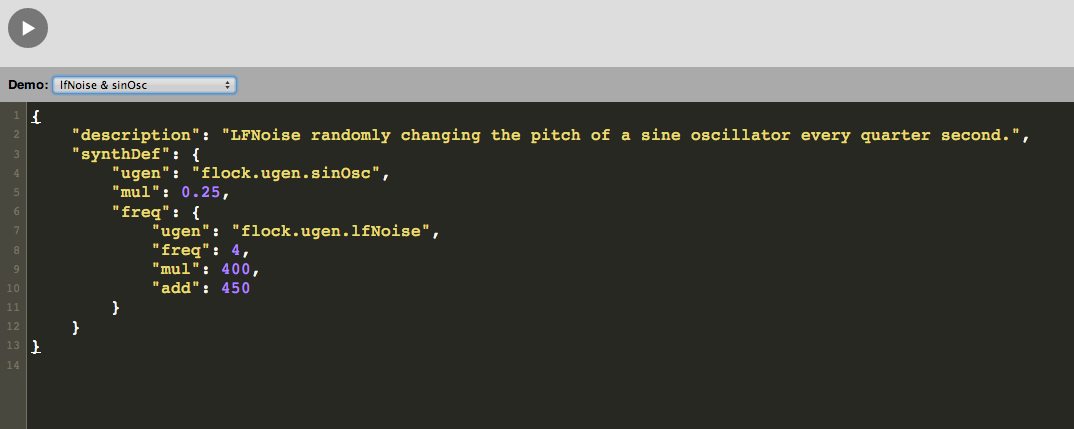
\includegraphics[width=0.9\columnwidth]{playground.png}
\caption{ A screenshot of the included interactive programming environment.\label{fig:playground}}
\end{figure}

\begin{figure}[h]
\centering
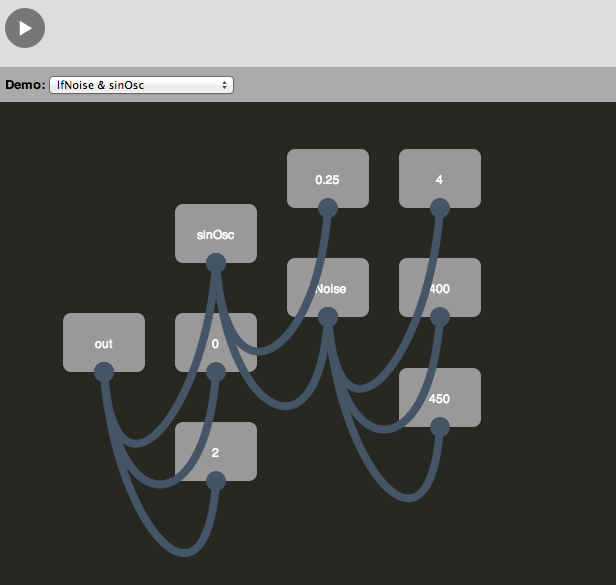
\includegraphics[width=0.9\columnwidth]{graphical.png}
\caption{ A screenshot of a patching GUI for Flocking.\label{fig:graphical}}
\end{figure}


\section{Next Steps}

\begin{itemize}
  \item Improve the the declarative scheduler's ability to schedule a variety of events efficiently, including the ability to inject sample-accurate changes into the main signal graph
  \item A new Flocking development environment that allows synths to be edited both as JSON and graphically with boxes and wires
  \item Web Audio ``islands," enabling users to freely interleave Flocking unit generators with native Web Audio nodes
\end{itemize}

%\section{Floats and equations}

%\subsection{Equations}
%Equations should be placed on separated lines and numbered.
%The number should be on the right side, in parentheses.
%\begin{equation}
%E=mc^{2}.
%\label{eq:Emc2}
%\end{equation}

%\pagebreak

%\subsection{Figures, Tables and Captions}
%All artwork must be centered, neat, clean, and legible. All lines should be very dark for purposes of reproduction and artwork should not be hand-drawn. The proceedings will be distributed in electronic form only, therefore color figures are allowed. However, you may want to check that your figures are understandable even if they are printed in black-and-white.
%\begin{table}[h]
% \begin{center}
% \begin{tabular}{|l|l|}
%  \hline
%  String value & Numeric value \\
%  \hline
%  Hello ICMC SMC  & 2014 \\
%  \hline
% \end{tabular}
%\end{center}
% \caption{Table captions should be placed below the table.}
% \label{tab:example}
%\end{table}

%Numbers and captions of figures and tables always appear below the figure/table. Leave 1 line space between the figure or table and the caption. Figure and tables are numbered consecutively. Captions should be Times 10~pt. Place tables/figures in text as close to the reference as possible, and preferably at the top of the page.

%\begin{figure}[h]
%\centering
%\includegraphics[width=0.9\columnwidth]{Athens_University_main_building.pdf}
%\caption{Figure captions should be placed below the figure,
%exactly like this.
%This photo shows the main building of the University of Athens.\label{fig:example}}
%\end{figure}

%Always refer to tables and figures in the main text, for example:
%see Figure \ref{fig:example} and \tabref{tab:example}.

%\begin{figure}[t]
%\figbox{
%\subfloat[][]{\includegraphics[width=60mm]{figure}\label{fig:subfigex_a}}\\
%\subfloat[][]{\includegraphics[width=80mm]{figure}\label{fig:subfigex_b}}
%}
%\caption{Here's an example using the subfig package.\label{fig:subfigex} }
%\end{figure}



\section{Conclusions}
Awesomeness has been demonstrated.

\nocite{*} % just to put everything in reference section for now

\begin{acknowledgments}
Funding agencies? Pets?
\end{acknowledgments}

%%%%%%%%%%%%%%%%%%%%%%%%%%%%%%%%%%%%%%%%%%%%%%%%%%%%%%%%%%%%%%%%%%%%%%%%%%%%%
%bibliography here
\bibliography{flockingbibliography}

\end{document}
